% % ANEXO------------------------------------------------------------------------

\begin{anexosenv}
\partanexos

% % Primeiro anexo---------------------------------------------------------------
\chapter{Formulário do produtor}     % edite para alterar o título deste anexo
\label{chap:anexoA}

\begin{figure}[!htb]
    \centering
    \caption{Formulário de mortalidade e ração recebida}
    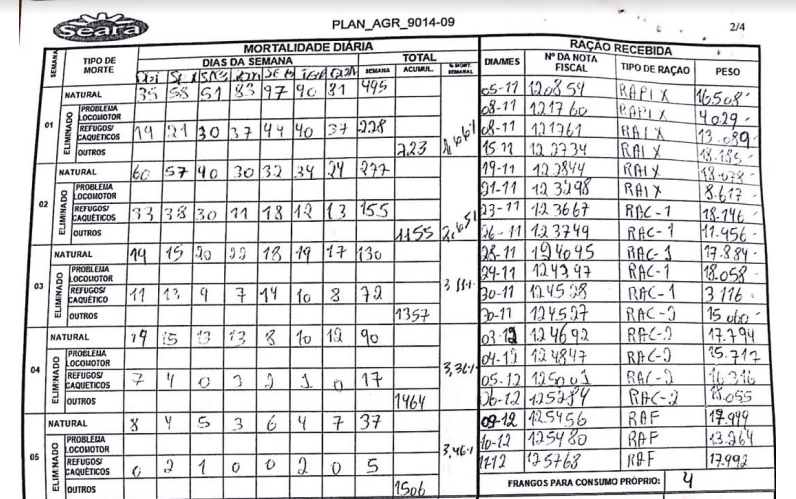
\includegraphics[width=1.0\textwidth]{./dados/figuras/planilha_mortalidade.png}
    \fonte{Autor}
    \label{fig:planilha_mortalidade}
\end{figure}

% Lembre-se que a diferença entre apêndice e anexo diz respeito à autoria do texto e/ou material ali colocado.

% Caso o material ou texto suplementar ou complementar seja de sua autoria, então ele deverá ser colocado como um apêndice. Porém, caso a autoria seja de terceiros, então o material ou texto deverá ser colocado como anexo.

% Caso seja conveniente, podem ser criados outros anexos para o seu trabalho acadêmico. Basta recortar e colar este trecho neste mesmo documento. Lembre-se de alterar o "label"{} do anexo.

% Organize seus anexos de modo a que, em cada um deles, haja um único tipo de conteúdo. Isso facilita a leitura e compreensão para o leitor do trabalho. É para ele que você escreve.

% % % Novo anexo-------------------------------------------------------------------
% \chapter{Nome do outro anexo}
% \label{chap:anexoB}

% \begin{figure}[!htb]
%     \centering
%     \caption{Peso médio do lote}
%     \includegraphics[width=1.0\textwidth]{./dados/figuras/pesagem_lote.png}
%     \fonte{Autor}
%     \label{fig:pesagem_lote}
% \end{figure}

\end{anexosenv}
